\documentclass[UTF8]{ctexart}
%字体配置
%\documentclass[UTF8]{ctexreport}
%以上是报告版,可以添加章节
%这里可以书写注释
\usepackage{graphicx}
\usepackage{caption}
\usepackage{subfigure}
\usepackage{float}
\usepackage{cite}
\usepackage{url}
%以上是使用图形包(傻瓜加入完事了)

\title{人机工学:个人调查报告}
\author{陈禹汀}
\date{2020/10/3}
%以上为文章属性设置
\begin{document}

\maketitle%自动制作标题
\newpage
\tableofcontents%生成目录
\newpage
%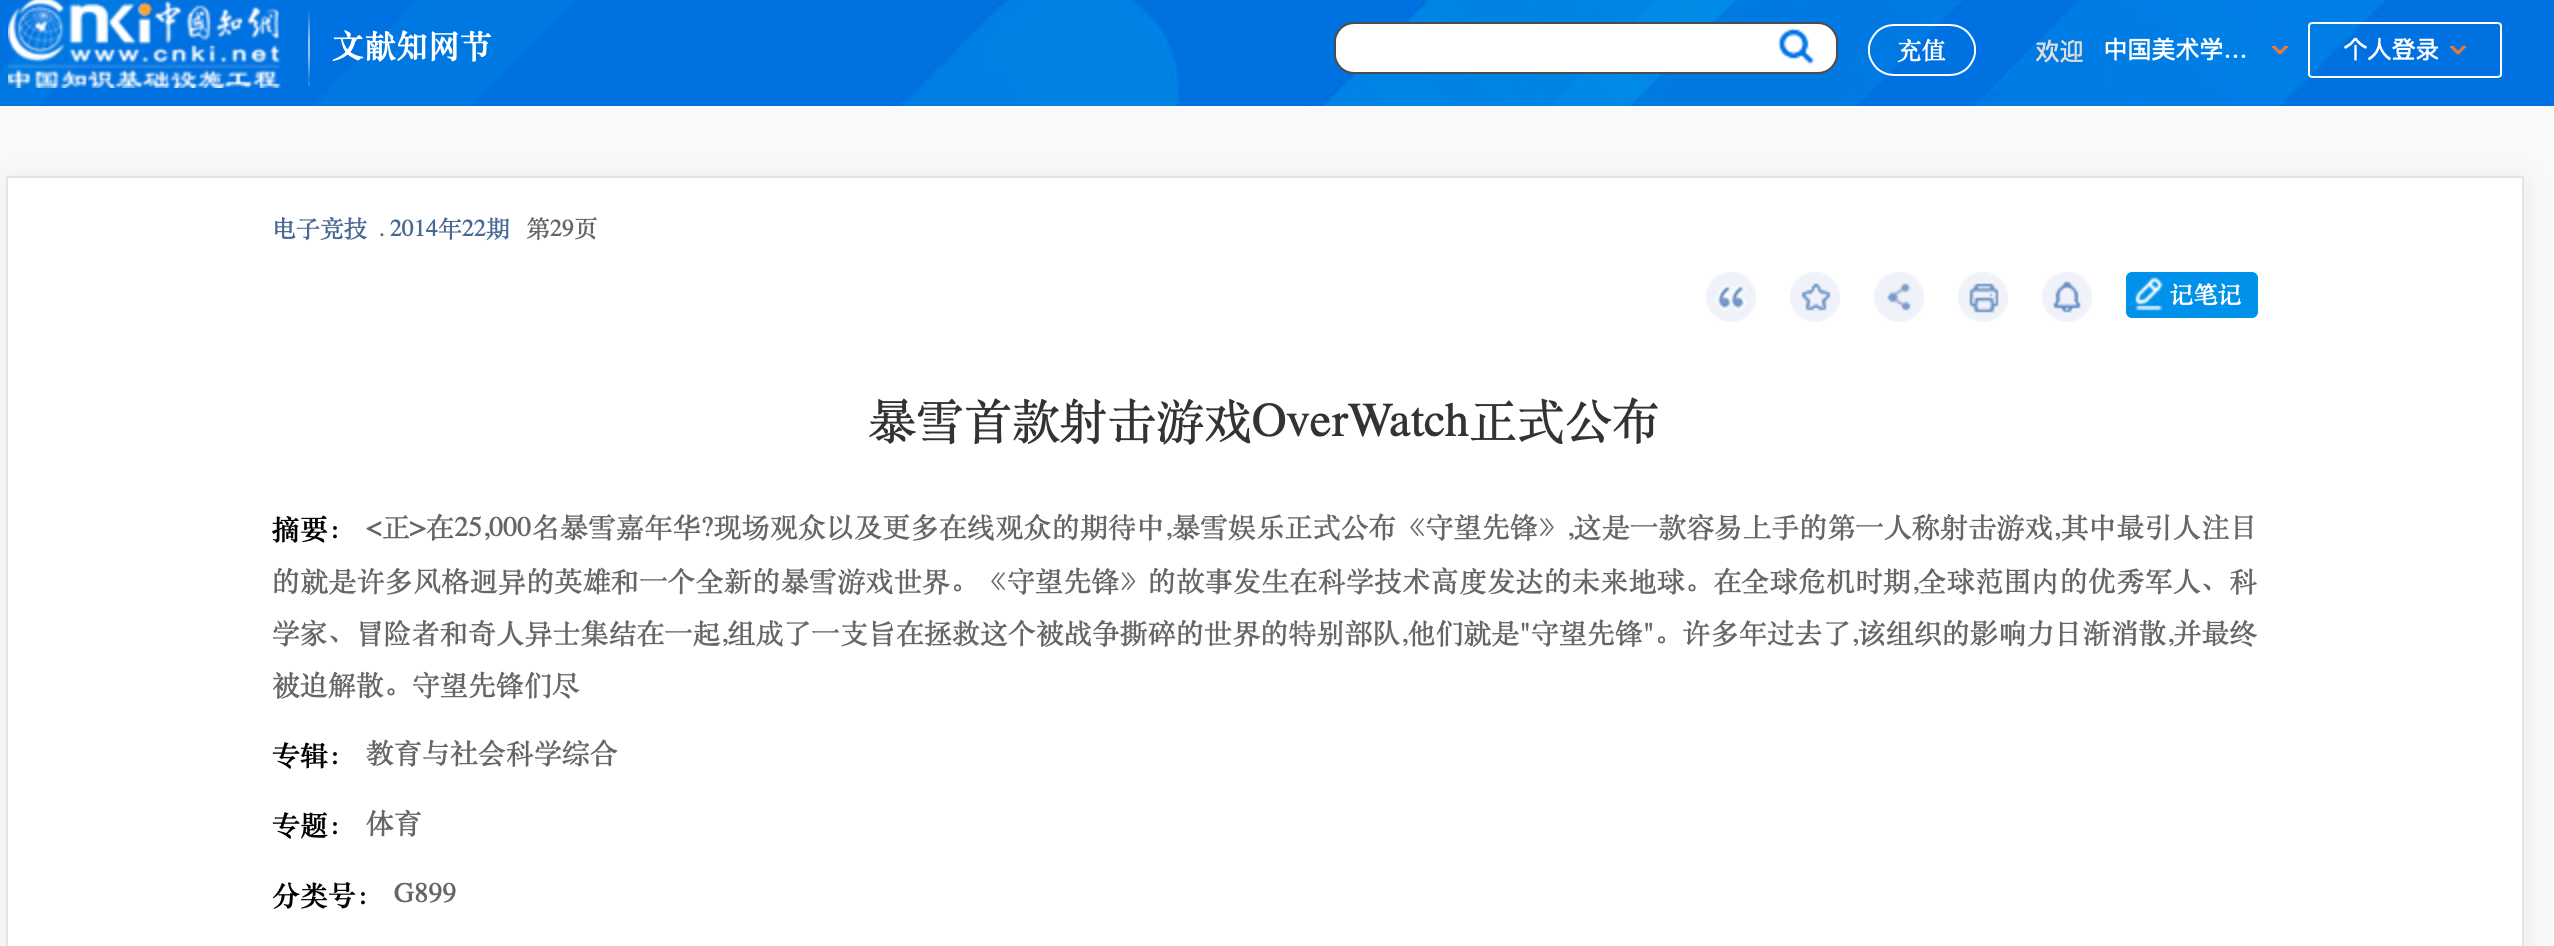
\includegraphics[width = .8\textwidth]{1.png}
%以上是插入图片
\section{个人调研}
    本次人机工学个人小作业调研的方向是电子竞技(主要游戏设备为个人电脑,主要游戏为《守望先锋》)中人体的动态。
\subsection{为什么是PC电子竞技?}
\paragraph{社会趋势}
    电子竞技正逐渐变成人类进行消遣行为的一种主要方式。"2020年突发疫情改变了人们文化消费的方式与内容,直接影响到生产端供给,以网络游戏、在线观影、短视频等为代表的数字文创产业成为文化消费的主力军." \cite{esports}
\paragraph{使用条件}
    虽然电子游戏的依附终端从比较难以携带的个人主机已经逐渐变到几乎成为“义肢”的智能手机。但是移动设备无法满足高强度的持续运行,以及高帧率高画质的性能,然而fps游戏往往需要这些性能来进行平滑的影像处理。 \cite{framerate}所以当前主要的大型电子竞技游戏平台依然是桌面端.

\subsection{为什么是《守望先锋》}
    守望先锋是一款结合fps和MOBA类风格的游戏,它像是《英雄联盟》、《DOTA2》这些MOBA类游戏,存在着高APM的操作 \cite{wiki:APM}。同时它也需要拥有《CS:GO》《战地(系列)》中准确瞄准能力。因而这是一款非常具有样本性的一款游戏。我们能够从它的操作行为模式中获取人与电子竞技类游戏之间的关系。

\section{数据获取以及筛选}
\paragraph{职业赛场}
    从不少的网站上可以仔细地查看到各大职业选手的鼠标和设备参数,我们能够从这些样本中获取不少信息。从prosettings网站上我们可以迅速地查阅到联赛选手和twitch主播的设置。 \cite{prosetting_edpi}在其中需要得到我们注重的是他们使用的鼠标、eDPI(灵敏度*鼠标DPI)以及与之成反比的360度转身鼠标转动距离。 \cite{prosetting_guide}这样我们能够统计出职业选手的普遍转动距离作为初步参考。

    \begin{figure}[h]
        \centering
        \includegraphics{pics/prosettings.png}
        \caption{Elliptic Paraboloid}
        \label{1}
    \end{figure} 

\bibliographystyle{ieeetr}
\bibliography{myref}    

\end{document}

